% main.tex
\documentclass{Report} % 使用您自定义的类

% --- 设置所有封面和页眉的占位符信息 ---
\ReportLogo{ZJU.jpg} % 您的代码指定了 ZJU.jpg
\Major{信息工程}
\StudentName{何~铭~源}
\StudentID{3240104481}
\ReportDate{\today}
\ReportLocation{紫金港东四219}

\CourseName{电子电路设计实验I}
\TeacherName{施红军、叶险峰、邓靖靖}
\ExperimentName{基尔霍夫定律的实验研究} % 此项也会用于页眉
\ExperimentType{验证类实验}
\TeamMate{孙潇枫}

\begin{document}


\makecover

\section{实验目的}
\begin{enumerate}
    \item 定量验证基尔霍夫电流定律（KCL）和基尔霍夫电压定律（KVL）在直流电路中的正确性。并加深对电路理论的理解。

    \item 掌握直流电路的基本连接、电压和电流的测量方法。

    \item 加深理解基尔霍夫定律是电路中电荷守恒和能量守恒原理的具体体现。

    \item 熟悉复杂电路的分析方法，培养实验动手能力和数据处理能力。
\end{enumerate}

\section{实验任务和要求}
\begin{enumerate}
    \item 使用理论计算出电路中各个支路的电流值与各个节点的电压值
    \item 使用电流表，电压表测量实际值，并与理论值进行对比，验证KCL，KVL的正确性
\end{enumerate}
\section{实验原理}
基尔霍夫定律：测量某电路中的各支路电流及每个元件两端的电压，应分别满足基尔霍夫电流定律（KCL）
和电压定律（KVL）。
\begin{enumerate}
    \item KCL: 对电路中的任一个节点而言
    \begin{equation}
        \sum_{n=1}^{N} i_n = 0
    \end{equation}
    \item KVL: 对电路中的任何一个闭合回路而言
    \begin{equation}
        \sum_{n=1}^{N} u_n = 0
    \end{equation}
\end{enumerate}
运用上述定律时必须设定各支路或闭合回路中电流的正方向。
\section{实验方案设计与参数计算}
\subsection{实验方案总体设计}
\begin{figure}[H]
\centering
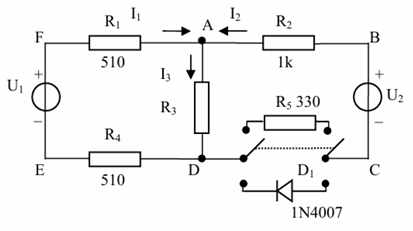
\includegraphics[width=0.6\textwidth]{./fig/基尔霍夫.png}
\caption{设计电路验证KCL，KVL}
\end{figure}
本次实验的核心目的是利用图1所示的电路，来对基尔霍夫定律（KCL和KVL）进行实验验证。
在开始测量之前，我们首先需要明确电路分析的参考方向。
对于三个主要的支路电流，我们遵循图1中已标明（$I_1, I_2, I_3$）的方向。
同时，我们选取了三个闭合回路（ADEFA、BADCB 和 FBCEF）作为分析对象，并设定了它们各自的绕行正方向。
实验中，我们采用了两路直流稳压电源接入电路，并将它们的输出电压均设定为 6V（即 $U_{s1} = U_{s2} = 6V$）。
具体的实验步骤分为以下两部分：
\begin{enumerate}
    \item \textbf{电阻情况：} 首先，将电阻 $R_5$ 接入指定电路位置，待电路稳定后，测量并记录相关的电压和电流读数。
    \item \textbf{二极管情况：} 接着，我们将 $R_5$ 替换为二极管 $D_1$，保持电源电压不变，重复上述测量步骤，并记录此时的数据。
\end{enumerate}
\subsection{理论值计算}
\subsubsection{$R_5$ 接入情况：支路电流}
根据基尔霍夫定律（KVL与KCL）列出方程组：

\begin{equation}
    \begin{cases}
    1020I_1 + 510I_3 = 6 \\
    1330I_2 + 510I_3 = 12 \\
    I_1 + I_2 = I_3
    \end{cases}
\label{eq:R}
\end{equation}


求解方程组\cref{eq:R}可得：
\begin{equation}
    \begin{cases}
    I_1 = 2.298\,mA \\
    I_2 = 6.325\,mA \\
    I_3 = 8.623\,mA
    \end{cases}
\end{equation}
\subsubsection{$D_1$ 接入情况：支路电流}
当二极管 $D_1$ 接入，理想模型下 $I_2 = 0$，此时 $I_1 = I_3$。方程组 (1) 简化为：
\begin{equation}
\begin{cases}
1020I_1 + 510I_3 = 6 \\
I_1 = I_3 \\
I_2 = 0
\end{cases}
\label{eq:D}
\end{equation}
求解方程\cref{eq:D}可得：
\begin{equation}
\begin{cases}
I_1 = 3.922\,mA \\
I_2 = 0\,mA \\
I_3 = 3.922\,mA
\end{cases}
\end{equation}

根据已求出的电流值，可进一步计算 $U_1, U_2, U_{FA}, U_{AB}, U_{AD}, U_{CD}, U_{DE}$ 等各点电位。
\section{实验仪器设备}
\begin{itemize}
    \item 万用表
    \item 电流表
    \item 实验室提供的电路板
\end{itemize}
\section{实验步骤、实验数据记录}
\subsection{电流值}

先将 $R_5$ 接入电路，测量电流值

\begin{table}[H] % [htbp] 允许表格浮动到合适的位置
    \centering % 表格居中
    \caption{各支路电流测量值}
    \begin{tabular}{lccc}
        \toprule
                   & $I_1$ (mA) & $I_2$ (mA) & $I_3$ (mA) \\
        \midrule
        计算值 & 1.926      & 5.988      & 7.914      \\
        测量值 & 1.92       & 5.81       & 7.84       \\
        \bottomrule
    \end{tabular}
\end{table}

可以发现，$I_1 + I_2 \approx I_3$，即验证了基尔霍夫电流定律成立。

\medskip % 增加一点垂直间距
再将 $D_1$ 接入电路，测量电流值

\begin{table}[H]
    \centering
    \caption{各支路电流测量值}
    \begin{tabular}{lccc}
        \toprule
                   & $I_1$ (mA) & $I_2$ (mA) & $I_3$ (mA) \\
        \midrule
        计算值 & 3.922      & 0          & 3.922      \\
        测量值 & 3.97       & 0          & 3.93       \\
        \bottomrule
    \end{tabular}
\end{table}

\subsection{电压值}

将 $R_5$ 接入电路，测量各节点的电压值

\begin{table}[H]
    \centering
    \caption{各节点电压测量值}
    \begin{tabular}{lccccccc}
        \toprule
                   & $U_1$  & $U_2$  & $U_{FA}$ & $U_{AB}$ & $U_{AD}$ & $U_{CD}$ & $U_{DE}$ \\
        \midrule
        理论值 & 6V     & 12V    & 0.982V   & -5.988V  & 4.036V   & -1.995V  & 0.982V   \\
        测量值 & 6.01V  & 11.94V & 1.00V    & -5.95V   & 3.96V    & -2.01V   & 1.03V    \\
        \bottomrule
    \end{tabular}
\end{table}

满足 $\sum U = 0$，验证了基尔霍夫电压定律成立。

\medskip
将 $D_1$ 接入电路，测量各节点的电压值

\begin{table}[H]
    \centering
    \caption{各节点电压测量值}
    \begin{tabular}{lccccccc}
        \toprule
                   & $U_1$  & $U_2$  & $U_{FA}$ & $U_{AB}$ & $U_{AD}$ & $U_{CD}$ & $U_{DE}$ \\
        \midrule
        理论值 & 6V     & 12V    & 2V       & 0V       & 2V       & -10V     & 2V       \\
        测量值 & 6.00V  & 12.01V & 1.97V    & 0V       & 1.98V    & -10.03V  & 2.03V    \\
        \bottomrule
    \end{tabular}
\end{table}

满足 $\sum U = 0$，即验证了对于非线性元件，基尔霍夫电压定律仍然成立。

\section{数据分析与讨论}
\begin{enumerate}
    \item \textbf{KCL 验证：} 无论是在 $R_5$ 线性电路还是 $D_1$非线性电路中，各支路电流的测量值均与理论值符合较好，验证了基尔霍夫电流定律。
    \item \textbf{KVL 验证：} 所有电路中的电压测量值也与理论值基本吻合（$\sum U \approx 0$），验证了基尔霍夫电压定律。
    \item \textbf{非线性适用性：} $D_1$ 电路中 $I_2$ 的理论与实测值均为0，有力证明了基尔霍夫定律对非线性元件同样有效。
    \item \textbf{误差分析：} 实验数据与理论值存在微小偏差，此误差在可接受范围内，表明实验方法和设备具有较高的准确性。
\end{enumerate}

\section{结论}
基尔霍夫电流定律和电压定律成立，即
\begin{align}
    \sum I_\text{in} = \sum I_\text{out}\\
    \sum U = 0.
\end{align}

\section{心得与体会}

通过本次实验，我成功验证了基尔霍夫定律在实际电路中的准确性。
这不仅加深了我对电路分析基本法则（电荷守恒与能量守恒）的理解，也显著提升了我的电路搭建与测量的实践操作能力。

\section{思考题}

\begin{enumerate}

    \item \textbf{如果设定不同的电压与电流参考方向，基尔霍夫定律是否仍然成立？}

    \textbf{答：仍然成立。}

    基尔霍夫定律描述的是电路中物理量的\textbf{代数和}关系，其成立与否不依赖于人为设定的参考方向，KCL，KVL实际上是电荷守恒和能量守恒的一种表达。

    \begin{itemize}
        \item \textbf{KCL（电流定律）：} KCL 表明“流入节点的电流代数和为零”。参考方向的选择只会影响表达式中各项的正负号，但总和恒为零的物理事实不会改变。
        \item \textbf{KVL（电压定律）：} KVL 表明“沿任一回路的电压代数和为零”。同理，参考方向的改变只会让回路方程中所有项的正负号统一反转，总和依然为零。
    \end{itemize}

    \item \textbf{如果电路中含有非线性器件，基尔霍夫定律是否仍然成立？}

    \textbf{答：依旧成立。}

    基尔霍夫定律的物理基础是电荷守恒和能量守恒，这两条是普适的物理定律，它们不依赖于电路元件的具体特性。

    \begin{itemize}
        \item \textbf{KCL（电流定律）}源于\textbf{电荷守恒}，即任一节点上的电荷不能凭空产生或消失。
        \item \textbf{KVL（电压定律）}源于\textbf{能量守恒}，即电荷绕回路一周所获得的能量必定等于其失去的能量。
    \end{itemize}

    无论元件是线性的（如电阻）还是非线性的（如本实验中的二极管 $D_1$），电流和电压都必须遵守这两条基本守恒定律。因此，基尔霍夫定律对非线性电路同样完全适用。

\end{enumerate}
\end{document}